\documentclass[1p]{elsarticle_modified}
%\bibliographystyle{elsarticle-num}

%\usepackage[colorlinks]{hyperref}
%\usepackage{abbrmath_seonhwa} %\Abb, \Ascr, \Acal ,\Abf, \Afrak
\usepackage{amsfonts}
\usepackage{amssymb}
\usepackage{amsmath}
\usepackage{amsthm}
\usepackage{scalefnt}
\usepackage{amsbsy}
\usepackage{kotex}
\usepackage{caption}
\usepackage{subfig}
\usepackage{color}
\usepackage{graphicx}
\usepackage{xcolor} %% white, black, red, green, blue, cyan, magenta, yellow
\usepackage{float}
\usepackage{setspace}
\usepackage{hyperref}

\usepackage{tikz}
\usetikzlibrary{arrows}

\usepackage{multirow}
\usepackage{array} % fixed length table
\usepackage{hhline}

%%%%%%%%%%%%%%%%%%%%%
\makeatletter
\renewcommand*\env@matrix[1][\arraystretch]{%
	\edef\arraystretch{#1}%
	\hskip -\arraycolsep
	\let\@ifnextchar\new@ifnextchar
	\array{*\c@MaxMatrixCols c}}
\makeatother %https://tex.stackexchange.com/questions/14071/how-can-i-increase-the-line-spacing-in-a-matrix
%%%%%%%%%%%%%%%

\usepackage[normalem]{ulem}

\newcommand{\msout}[1]{\ifmmode\text{\sout{\ensuremath{#1}}}\else\sout{#1}\fi}
%SOURCE: \msout is \stkout macro in https://tex.stackexchange.com/questions/20609/strikeout-in-math-mode

\newcommand{\cancel}[1]{
	\ifmmode
	{\color{red}\msout{#1}}
	\else
	{\color{red}\sout{#1}}
	\fi
}

\newcommand{\add}[1]{
	{\color{blue}\uwave{#1}}
}

\newcommand{\replace}[2]{
	\ifmmode
	{\color{red}\msout{#1}}{\color{blue}\uwave{#2}}
	\else
	{\color{red}\sout{#1}}{\color{blue}\uwave{#2}}
	\fi
}

\newcommand{\Sol}{\mathcal{S}} %segment
\newcommand{\D}{D} %diagram
\newcommand{\A}{\mathcal{A}} %arc


%%%%%%%%%%%%%%%%%%%%%%%%%%%%%5 test

\def\sl{\operatorname{\textup{SL}}(2,\Cbb)}
\def\psl{\operatorname{\textup{PSL}}(2,\Cbb)}
\def\quan{\mkern 1mu \triangleright \mkern 1mu}

\theoremstyle{definition}
\newtheorem{thm}{Theorem}[section]
\newtheorem{prop}[thm]{Proposition}
\newtheorem{lem}[thm]{Lemma}
\newtheorem{ques}[thm]{Question}
\newtheorem{cor}[thm]{Corollary}
\newtheorem{defn}[thm]{Definition}
\newtheorem{exam}[thm]{Example}
\newtheorem{rmk}[thm]{Remark}
\newtheorem{alg}[thm]{Algorithm}

\newcommand{\I}{\sqrt{-1}}
\begin{document}

%\begin{frontmatter}
%
%\title{Boundary parabolic representations of knots up to 8 crossings}
%
%%% Group authors per affiliation:
%\author{Yunhi Cho} 
%\address{Department of Mathematics, University of Seoul, Seoul, Korea}
%\ead{yhcho@uos.ac.kr}
%
%
%\author{Seonhwa Kim} %\fnref{s_kim}}
%\address{Center for Geometry and Physics, Institute for Basic Science, Pohang, 37673, Korea}
%\ead{ryeona17@ibs.re.kr}
%
%\author{Hyuk Kim}
%\address{Department of Mathematical Sciences, Seoul National University, Seoul 08826, Korea}
%\ead{hyukkim@snu.ac.kr}
%
%\author{Seokbeom Yoon}
%\address{Department of Mathematical Sciences, Seoul National University, Seoul, 08826,  Korea}
%\ead{sbyoon15@snu.ac.kr}
%
%\begin{abstract}
%We find all boundary parabolic representation of knots up to 8 crossings.
%
%\end{abstract}
%\begin{keyword}
%    \MSC[2010] 57M25 
%\end{keyword}
%
%\end{frontmatter}

%\linenumbers
%\tableofcontents
%
\newcommand\colored[1]{\textcolor{white}{\rule[-0.35ex]{0.8em}{1.4ex}}\kern-0.8em\color{red} #1}%
%\newcommand\colored[1]{\textcolor{white}{ #1}\kern-2.17ex	\textcolor{white}{ #1}\kern-1.81ex	\textcolor{white}{ #1}\kern-2.15ex\color{red}#1	}

{\Large $\underline{12a_{1083}~(K12a_{1083})}$}

\setlength{\tabcolsep}{10pt}
\renewcommand{\arraystretch}{1.6}
\vspace{1cm}\begin{tabular}{m{100pt}>{\centering\arraybackslash}m{274pt}}
\multirow{5}{120pt}{
	\centering
	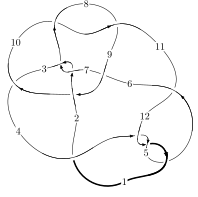
\includegraphics[width=112pt]{../../../GIT/diagram.site/Diagrams/png/1884_12a_1083.png}\\
\ \ \ A knot diagram\footnotemark}&
\allowdisplaybreaks
\textbf{Linearized knot diagam} \\
\cline{2-2}
 &
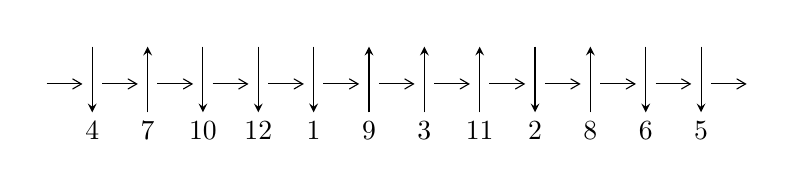
\begin{tikzpicture}[x=20pt, y=17pt]
	% nodes
	\node (C0) at (0, 0) {};
	\node (C1) at (1, 0) {};
	\node (C1U) at (1, +1) {};
	\node (C1D) at (1, -1) {4};

	\node (C2) at (2, 0) {};
	\node (C2U) at (2, +1) {};
	\node (C2D) at (2, -1) {7};

	\node (C3) at (3, 0) {};
	\node (C3U) at (3, +1) {};
	\node (C3D) at (3, -1) {10};

	\node (C4) at (4, 0) {};
	\node (C4U) at (4, +1) {};
	\node (C4D) at (4, -1) {12};

	\node (C5) at (5, 0) {};
	\node (C5U) at (5, +1) {};
	\node (C5D) at (5, -1) {1};

	\node (C6) at (6, 0) {};
	\node (C6U) at (6, +1) {};
	\node (C6D) at (6, -1) {9};

	\node (C7) at (7, 0) {};
	\node (C7U) at (7, +1) {};
	\node (C7D) at (7, -1) {3};

	\node (C8) at (8, 0) {};
	\node (C8U) at (8, +1) {};
	\node (C8D) at (8, -1) {11};

	\node (C9) at (9, 0) {};
	\node (C9U) at (9, +1) {};
	\node (C9D) at (9, -1) {2};

	\node (C10) at (10, 0) {};
	\node (C10U) at (10, +1) {};
	\node (C10D) at (10, -1) {8};

	\node (C11) at (11, 0) {};
	\node (C11U) at (11, +1) {};
	\node (C11D) at (11, -1) {6};

	\node (C12) at (12, 0) {};
	\node (C12U) at (12, +1) {};
	\node (C12D) at (12, -1) {5};
	\node (C13) at (13, 0) {};

	% arrows
	\draw[->,>={angle 60}]
	(C0) edge (C1) (C1) edge (C2) (C2) edge (C3) (C3) edge (C4) (C4) edge (C5) (C5) edge (C6) (C6) edge (C7) (C7) edge (C8) (C8) edge (C9) (C9) edge (C10) (C10) edge (C11) (C11) edge (C12) (C12) edge (C13) ;	\draw[->,>=stealth]
	(C1U) edge (C1D) (C2D) edge (C2U) (C3U) edge (C3D) (C4U) edge (C4D) (C5U) edge (C5D) (C6D) edge (C6U) (C7D) edge (C7U) (C8D) edge (C8U) (C9U) edge (C9D) (C10D) edge (C10U) (C11U) edge (C11D) (C12U) edge (C12D) ;
	\end{tikzpicture} \\
\hhline{~~} \\& 
\textbf{Solving Sequence} \\ \cline{2-2} 
 &
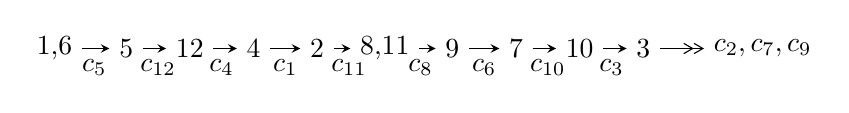
\begin{tikzpicture}[x=23pt, y=7pt]
	% node
	\node (A0) at (-1/8, 0) {1,6};
	\node (A1) at (1, 0) {5};
	\node (A2) at (2, 0) {12};
	\node (A3) at (3, 0) {4};
	\node (A4) at (4, 0) {2};
	\node (A5) at (81/16, 0) {8,11};
	\node (A6) at (49/8, 0) {9};
	\node (A7) at (57/8, 0) {7};
	\node (A8) at (65/8, 0) {10};
	\node (A9) at (73/8, 0) {3};
	\node (C1) at (1/2, -1) {$c_{5}$};
	\node (C2) at (3/2, -1) {$c_{12}$};
	\node (C3) at (5/2, -1) {$c_{4}$};
	\node (C4) at (7/2, -1) {$c_{1}$};
	\node (C5) at (9/2, -1) {$c_{11}$};
	\node (C6) at (45/8, -1) {$c_{8}$};
	\node (C7) at (53/8, -1) {$c_{6}$};
	\node (C8) at (61/8, -1) {$c_{10}$};
	\node (C9) at (69/8, -1) {$c_{3}$};
	\node (A10) at (11, 0) {$c_{2},c_{7},c_{9}$};

	% edge
	\draw[->,>=stealth]	
	(A0) edge (A1) (A1) edge (A2) (A2) edge (A3) (A3) edge (A4) (A4) edge (A5) (A5) edge (A6) (A6) edge (A7) (A7) edge (A8) (A8) edge (A9) ;
	\draw[->>,>={angle 60}]	
	(A9) edge (A10);
\end{tikzpicture} \\ 

\end{tabular} \\

\footnotetext{
The image of knot diagram is generated by the software ``\textbf{Draw programme}" developed by Andrew Bartholomew(\url{http://www.layer8.co.uk/maths/draw/index.htm\#Running-draw}), where we modified some parts for our purpose(\url{https://github.com/CATsTAILs/LinksPainter}).
}\phantom \\ \newline 
\centering \textbf{Ideals for irreducible components\footnotemark of $X_{\text{par}}$} 
 
\begin{align*}
I^u_{1}&=\langle 
-2.11665\times10^{47} u^{88}-1.10564\times10^{47} u^{87}+\cdots+6.92682\times10^{46} b-2.35140\times10^{47},\\
\phantom{I^u_{1}}&\phantom{= \langle  }3.99720\times10^{45} u^{88}-1.09937\times10^{45} u^{87}+\cdots+6.29711\times10^{45} a+7.42531\times10^{45},\;u^{89}+2 u^{88}+\cdots- u+1\rangle \\
I^u_{2}&=\langle 
2 u^4-12 u^3+7 b+9 u+6,\;- u^4- u^3+7 a+6 u-3,\;u^5- u^4-2 u^3+u^2+u+1\rangle \\
\\
\end{align*}
\raggedright * 2 irreducible components of $\dim_{\mathbb{C}}=0$, with total 94 representations.\\
\footnotetext{All coefficients of polynomials are rational numbers. But the coefficients are sometimes approximated in decimal forms when there is not enough margin.}
\newpage
\renewcommand{\arraystretch}{1}
\centering \section*{I. $I^u_{1}= \langle -2.12\times10^{47} u^{88}-1.11\times10^{47} u^{87}+\cdots+6.93\times10^{46} b-2.35\times10^{47},\;4.00\times10^{45} u^{88}-1.10\times10^{45} u^{87}+\cdots+6.30\times10^{45} a+7.43\times10^{45},\;u^{89}+2 u^{88}+\cdots- u+1 \rangle$}
\flushleft \textbf{(i) Arc colorings}\\
\begin{tabular}{m{7pt} m{180pt} m{7pt} m{180pt} }
\flushright $a_{1}=$&$\begin{pmatrix}0\\u\end{pmatrix}$ \\
\flushright $a_{6}=$&$\begin{pmatrix}1\\0\end{pmatrix}$ \\
\flushright $a_{5}=$&$\begin{pmatrix}1\\- u^2\end{pmatrix}$ \\
\flushright $a_{12}=$&$\begin{pmatrix}u\\- u^3+u\end{pmatrix}$ \\
\flushright $a_{4}=$&$\begin{pmatrix}- u^2+1\\u^4-2 u^2\end{pmatrix}$ \\
\flushright $a_{2}=$&$\begin{pmatrix}- u^5+2 u^3- u\\u^7-3 u^5+2 u^3+u\end{pmatrix}$ \\
\flushright $a_{8}=$&$\begin{pmatrix}-0.634768 u^{88}+0.174583 u^{87}+\cdots+7.02674 u-1.17916\\3.05573 u^{88}+1.59617 u^{87}+\cdots-5.89150 u+3.39464\end{pmatrix}$ \\
\flushright $a_{11}=$&$\begin{pmatrix}- u^3+2 u\\- u^3+u\end{pmatrix}$ \\
\flushright $a_{9}=$&$\begin{pmatrix}-0.126780 u^{88}+0.404435 u^{87}+\cdots+8.42304 u-0.381113\\1.69946 u^{88}+0.554035 u^{87}+\cdots-3.03296 u+2.56541\end{pmatrix}$ \\
\flushright $a_{7}=$&$\begin{pmatrix}3.16567 u^{88}+2.81717 u^{87}+\cdots-9.92028 u+0.927302\\-1.96936 u^{88}-2.61970 u^{87}+\cdots+6.37800 u-2.57339\end{pmatrix}$ \\
\flushright $a_{10}=$&$\begin{pmatrix}-0.388476 u^{88}+0.166599 u^{87}+\cdots+8.37411 u-0.515987\\1.83579 u^{88}+0.737421 u^{87}+\cdots-2.95142 u+2.51815\end{pmatrix}$ \\
\flushright $a_{3}=$&$\begin{pmatrix}-3.30265 u^{88}-3.44449 u^{87}+\cdots-0.682398 u-2.18348\\2.41903 u^{88}+3.69517 u^{87}+\cdots+1.98227 u+0.0416273\end{pmatrix}$\\&\end{tabular}
\flushleft \textbf{(ii) Obstruction class $= -1$}\\~\\
\flushleft \textbf{(iii) Cusp Shapes $= -6.44685 u^{88}-7.91516 u^{87}+\cdots+17.4108 u+0.723245$}\\~\\
\newpage\renewcommand{\arraystretch}{1}
\flushleft \textbf{(iv) u-Polynomials at the component}\newline \\
\begin{tabular}{m{50pt}|m{274pt}}
Crossings & \hspace{64pt}u-Polynomials at each crossing \\
\hline $$\begin{aligned}c_{1},c_{11}\end{aligned}$$&$\begin{aligned}
&u^{89}-6 u^{88}+\cdots-5907 u+847
\end{aligned}$\\
\hline $$\begin{aligned}c_{2},c_{7}\end{aligned}$$&$\begin{aligned}
&u^{89}+2 u^{88}+\cdots- u+1
\end{aligned}$\\
\hline $$\begin{aligned}c_{3}\end{aligned}$$&$\begin{aligned}
&7(7 u^{89}-109 u^{88}+\cdots-1197918 u-1021121)
\end{aligned}$\\
\hline $$\begin{aligned}c_{4},c_{5},c_{12}\end{aligned}$$&$\begin{aligned}
&u^{89}+2 u^{88}+\cdots- u+1
\end{aligned}$\\
\hline $$\begin{aligned}c_{6}\end{aligned}$$&$\begin{aligned}
&7(7 u^{89}+73 u^{88}+\cdots+4.22849\times10^{7} u+4324097)
\end{aligned}$\\
\hline $$\begin{aligned}c_{8},c_{10}\end{aligned}$$&$\begin{aligned}
&u^{89}+6 u^{88}+\cdots+1691 u+49
\end{aligned}$\\
\hline $$\begin{aligned}c_{9}\end{aligned}$$&$\begin{aligned}
&u^{89}-3 u^{88}+\cdots+59096 u^2-1568
\end{aligned}$\\
\hline
\end{tabular}\\~\\
\newpage\renewcommand{\arraystretch}{1}
\flushleft \textbf{(v) Riley Polynomials at the component}\newline \\
\begin{tabular}{m{50pt}|m{274pt}}
Crossings & \hspace{64pt}Riley Polynomials at each crossing \\
\hline $$\begin{aligned}c_{1},c_{11}\end{aligned}$$&$\begin{aligned}
&y^{89}+72 y^{88}+\cdots+9580901 y-717409
\end{aligned}$\\
\hline $$\begin{aligned}c_{2},c_{7}\end{aligned}$$&$\begin{aligned}
&y^{89}-60 y^{88}+\cdots-11 y-1
\end{aligned}$\\
\hline $$\begin{aligned}c_{3}\end{aligned}$$&$\begin{aligned}
&49\\
&\cdot(49 y^{89}-7919 y^{88}+\cdots-31244025855892 y-1042688096641)
\end{aligned}$\\
\hline $$\begin{aligned}c_{4},c_{5},c_{12}\end{aligned}$$&$\begin{aligned}
&y^{89}-72 y^{88}+\cdots-11 y-1
\end{aligned}$\\
\hline $$\begin{aligned}c_{6}\end{aligned}$$&$\begin{aligned}
&49\\
&\cdot(49 y^{89}-12749 y^{88}+\cdots+178083980700794 y-18697814865409)
\end{aligned}$\\
\hline $$\begin{aligned}c_{8},c_{10}\end{aligned}$$&$\begin{aligned}
&y^{89}-76 y^{88}+\cdots+3133195 y-2401
\end{aligned}$\\
\hline $$\begin{aligned}c_{9}\end{aligned}$$&$\begin{aligned}
&y^{89}+33 y^{88}+\cdots+185325056 y-2458624
\end{aligned}$\\
\hline
\end{tabular}\\~\\
\newpage\flushleft \textbf{(vi) Complex Volumes and Cusp Shapes}
$$\begin{array}{c|c|c}  
\text{Solutions to }I^u_{1}& \I (\text{vol} + \sqrt{-1}CS) & \text{Cusp shape}\\
 \hline 
\begin{aligned}
u &= \phantom{-}0.125382 + 0.878758 I \\
a &= -0.70658 + 2.95493 I \\
b &= -0.48390 + 2.47308 I\end{aligned}
 & \phantom{-}12.57200 - 0.58676 I & \phantom{-}7.92936 + 0. I\phantom{ +0.000000I} \\ \hline\begin{aligned}
u &= \phantom{-}0.125382 - 0.878758 I \\
a &= -0.70658 - 2.95493 I \\
b &= -0.48390 - 2.47308 I\end{aligned}
 & \phantom{-}12.57200 + 0.58676 I & \phantom{-}7.92936 + 0. I\phantom{ +0.000000I} \\ \hline\begin{aligned}
u &= -0.108009 + 0.878753 I \\
a &= \phantom{-}0.63992 + 3.41927 I \\
b &= \phantom{-}0.30080 + 2.77816 I\end{aligned}
 & \phantom{-}8.44721 + 6.94338 I & \phantom{-}3.88118 - 5.23404 I \\ \hline\begin{aligned}
u &= -0.108009 - 0.878753 I \\
a &= \phantom{-}0.63992 - 3.41927 I \\
b &= \phantom{-}0.30080 - 2.77816 I\end{aligned}
 & \phantom{-}8.44721 - 6.94338 I & \phantom{-}3.88118 + 5.23404 I \\ \hline\begin{aligned}
u &= \phantom{-}0.107640 + 0.869226 I \\
a &= -0.84277 + 3.64500 I \\
b &= -0.36192 + 3.00809 I\end{aligned}
 & \phantom{-}13.1823 - 12.7067 I & \phantom{-}5.61691 + 6.76212 I \\ \hline\begin{aligned}
u &= \phantom{-}0.107640 - 0.869226 I \\
a &= -0.84277 - 3.64500 I \\
b &= -0.36192 - 3.00809 I\end{aligned}
 & \phantom{-}13.1823 + 12.7067 I & \phantom{-}5.61691 - 6.76212 I \\ \hline\begin{aligned}
u &= -1.14112\phantom{ +0.000000I} \\
a &= -0.524359\phantom{ +0.000000I} \\
b &= -1.81639\phantom{ +0.000000I}\end{aligned}
 & \phantom{-}3.04390\phantom{ +0.000000I} & \phantom{-0.000000 } 0 \\ \hline\begin{aligned}
u &= -0.018538 + 0.839308 I \\
a &= -0.04785 - 3.30693 I \\
b &= \phantom{-}0.26758 - 2.88148 I\end{aligned}
 & \phantom{-}11.49580 + 2.45922 I & \phantom{-}9.88893 - 2.84321 I \\ \hline\begin{aligned}
u &= -0.018538 - 0.839308 I \\
a &= -0.04785 + 3.30693 I \\
b &= \phantom{-}0.26758 + 2.88148 I\end{aligned}
 & \phantom{-}11.49580 - 2.45922 I & \phantom{-}9.88893 + 2.84321 I \\ \hline\begin{aligned}
u &= \phantom{-}0.061352 + 0.829162 I \\
a &= -0.545645 - 0.852361 I \\
b &= -0.955134 - 0.749592 I\end{aligned}
 & \phantom{-}7.26203 - 6.26191 I & \phantom{-}5.35569 + 6.30354 I\\
 \hline 
 \end{array}$$\newpage$$\begin{array}{c|c|c}  
\text{Solutions to }I^u_{1}& \I (\text{vol} + \sqrt{-1}CS) & \text{Cusp shape}\\
 \hline 
\begin{aligned}
u &= \phantom{-}0.061352 - 0.829162 I \\
a &= -0.545645 + 0.852361 I \\
b &= -0.955134 + 0.749592 I\end{aligned}
 & \phantom{-}7.26203 + 6.26191 I & \phantom{-}5.35569 - 6.30354 I \\ \hline\begin{aligned}
u &= \phantom{-}0.014115 + 0.816635 I \\
a &= \phantom{-}1.52546 - 4.00461 I \\
b &= \phantom{-}0.82563 - 3.07082 I\end{aligned}
 & \phantom{-}6.78894 - 1.20316 I & \phantom{-}1.70987 + 0.75534 I \\ \hline\begin{aligned}
u &= \phantom{-}0.014115 - 0.816635 I \\
a &= \phantom{-}1.52546 + 4.00461 I \\
b &= \phantom{-}0.82563 + 3.07082 I\end{aligned}
 & \phantom{-}6.78894 + 1.20316 I & \phantom{-}1.70987 - 0.75534 I \\ \hline\begin{aligned}
u &= -0.061691 + 0.806346 I \\
a &= -0.245155 - 0.075307 I \\
b &= \phantom{-}0.214340 - 0.168825 I\end{aligned}
 & \phantom{-}3.54962 + 2.89056 I & -0.65715 - 3.47288 I \\ \hline\begin{aligned}
u &= -0.061691 - 0.806346 I \\
a &= -0.245155 + 0.075307 I \\
b &= \phantom{-}0.214340 + 0.168825 I\end{aligned}
 & \phantom{-}3.54962 - 2.89056 I & -0.65715 + 3.47288 I \\ \hline\begin{aligned}
u &= -0.517626 + 0.610535 I \\
a &= -1.32915 + 0.51384 I \\
b &= -0.251501 + 0.525803 I\end{aligned}
 & \phantom{-}2.17162 + 2.14937 I & \phantom{-}6.30599 - 5.13356 I \\ \hline\begin{aligned}
u &= -0.517626 - 0.610535 I \\
a &= -1.32915 - 0.51384 I \\
b &= -0.251501 - 0.525803 I\end{aligned}
 & \phantom{-}2.17162 - 2.14937 I & \phantom{-}6.30599 + 5.13356 I \\ \hline\begin{aligned}
u &= \phantom{-}0.034225 + 0.793430 I \\
a &= \phantom{-}2.62398 + 1.24253 I \\
b &= \phantom{-}1.60665 + 0.50390 I\end{aligned}
 & \phantom{-}6.48290 - 0.18025 I & \phantom{-}6.74425 - 0.95194 I \\ \hline\begin{aligned}
u &= \phantom{-}0.034225 - 0.793430 I \\
a &= \phantom{-}2.62398 - 1.24253 I \\
b &= \phantom{-}1.60665 - 0.50390 I\end{aligned}
 & \phantom{-}6.48290 + 0.18025 I & \phantom{-}6.74425 + 0.95194 I \\ \hline\begin{aligned}
u &= \phantom{-}1.22262\phantom{ +0.000000I} \\
a &= -0.570553\phantom{ +0.000000I} \\
b &= \phantom{-}2.43483\phantom{ +0.000000I}\end{aligned}
 & -1.22444\phantom{ +0.000000I} & \phantom{-0.000000 } 0\\
 \hline 
 \end{array}$$\newpage$$\begin{array}{c|c|c}  
\text{Solutions to }I^u_{1}& \I (\text{vol} + \sqrt{-1}CS) & \text{Cusp shape}\\
 \hline 
\begin{aligned}
u &= \phantom{-}1.140140 + 0.447012 I \\
a &= \phantom{-}1.56190 - 1.40744 I \\
b &= -0.75301 - 1.95426 I\end{aligned}
 & \phantom{-}9.46007 - 4.15016 I & \phantom{-0.000000 } 0 \\ \hline\begin{aligned}
u &= \phantom{-}1.140140 - 0.447012 I \\
a &= \phantom{-}1.56190 + 1.40744 I \\
b &= -0.75301 + 1.95426 I\end{aligned}
 & \phantom{-}9.46007 + 4.15016 I & \phantom{-0.000000 } 0 \\ \hline\begin{aligned}
u &= \phantom{-}1.221650 + 0.117112 I \\
a &= \phantom{-}0.542321 - 1.049280 I \\
b &= \phantom{-}0.744477 - 0.262187 I\end{aligned}
 & \phantom{-}1.49288 - 3.55667 I & \phantom{-0.000000 } 0 \\ \hline\begin{aligned}
u &= \phantom{-}1.221650 - 0.117112 I \\
a &= \phantom{-}0.542321 + 1.049280 I \\
b &= \phantom{-}0.744477 + 0.262187 I\end{aligned}
 & \phantom{-}1.49288 + 3.55667 I & \phantom{-0.000000 } 0 \\ \hline\begin{aligned}
u &= \phantom{-}0.537235 + 0.543423 I \\
a &= \phantom{-}1.43198 + 0.25042 I \\
b &= -0.017291 + 0.227081 I\end{aligned}
 & \phantom{-}6.94642 + 4.33545 I & \phantom{-}4.08323 - 1.64396 I \\ \hline\begin{aligned}
u &= \phantom{-}0.537235 - 0.543423 I \\
a &= \phantom{-}1.43198 - 0.25042 I \\
b &= -0.017291 - 0.227081 I\end{aligned}
 & \phantom{-}6.94642 - 4.33545 I & \phantom{-}4.08323 + 1.64396 I \\ \hline\begin{aligned}
u &= \phantom{-}1.160450 + 0.432770 I \\
a &= \phantom{-}1.78321 - 1.56494 I \\
b &= -0.68857 - 2.55744 I\end{aligned}
 & \phantom{-}9.95317 + 8.04672 I & \phantom{-0.000000 } 0 \\ \hline\begin{aligned}
u &= \phantom{-}1.160450 - 0.432770 I \\
a &= \phantom{-}1.78321 + 1.56494 I \\
b &= -0.68857 + 2.55744 I\end{aligned}
 & \phantom{-}9.95317 - 8.04672 I & \phantom{-0.000000 } 0 \\ \hline\begin{aligned}
u &= -1.161820 + 0.445584 I \\
a &= -1.73625 - 1.46920 I \\
b &= \phantom{-}0.57367 - 2.32260 I\end{aligned}
 & \phantom{-}5.21394 - 2.21357 I & \phantom{-0.000000 } 0 \\ \hline\begin{aligned}
u &= -1.161820 - 0.445584 I \\
a &= -1.73625 + 1.46920 I \\
b &= \phantom{-}0.57367 + 2.32260 I\end{aligned}
 & \phantom{-}5.21394 + 2.21357 I & \phantom{-0.000000 } 0\\
 \hline 
 \end{array}$$\newpage$$\begin{array}{c|c|c}  
\text{Solutions to }I^u_{1}& \I (\text{vol} + \sqrt{-1}CS) & \text{Cusp shape}\\
 \hline 
\begin{aligned}
u &= -1.24503\phantom{ +0.000000I} \\
a &= -0.621366\phantom{ +0.000000I} \\
b &= \phantom{-}0.809575\phantom{ +0.000000I}\end{aligned}
 & -2.34521\phantom{ +0.000000I} & \phantom{-0.000000 } 0 \\ \hline\begin{aligned}
u &= -1.254420 + 0.066692 I \\
a &= -0.296221 - 1.087230 I \\
b &= -0.450958 + 0.738893 I\end{aligned}
 & -2.36817 + 1.69929 I & \phantom{-0.000000 } 0 \\ \hline\begin{aligned}
u &= -1.254420 - 0.066692 I \\
a &= -0.296221 + 1.087230 I \\
b &= -0.450958 - 0.738893 I\end{aligned}
 & -2.36817 - 1.69929 I & \phantom{-0.000000 } 0 \\ \hline\begin{aligned}
u &= \phantom{-}0.473696 + 0.568911 I \\
a &= \phantom{-}1.032500 + 0.374017 I \\
b &= \phantom{-}0.033167 + 0.777124 I\end{aligned}
 & \phantom{-}7.13183 - 8.33264 I & \phantom{-}3.55448 + 7.75216 I \\ \hline\begin{aligned}
u &= \phantom{-}0.473696 - 0.568911 I \\
a &= \phantom{-}1.032500 - 0.374017 I \\
b &= \phantom{-}0.033167 - 0.777124 I\end{aligned}
 & \phantom{-}7.13183 + 8.33264 I & \phantom{-}3.55448 - 7.75216 I \\ \hline\begin{aligned}
u &= -1.215220 + 0.345432 I \\
a &= -0.321172 + 0.016545 I \\
b &= \phantom{-}0.022056 + 0.329477 I\end{aligned}
 & \phantom{-}0.013033 + 1.266560 I & \phantom{-0.000000 } 0 \\ \hline\begin{aligned}
u &= -1.215220 - 0.345432 I \\
a &= -0.321172 - 0.016545 I \\
b &= \phantom{-}0.022056 - 0.329477 I\end{aligned}
 & \phantom{-}0.013033 - 1.266560 I & \phantom{-0.000000 } 0 \\ \hline\begin{aligned}
u &= \phantom{-}1.210740 + 0.372378 I \\
a &= -0.344730 - 0.246031 I \\
b &= -0.644449 + 1.070780 I\end{aligned}
 & \phantom{-}3.72918 + 1.93529 I & \phantom{-0.000000 } 0 \\ \hline\begin{aligned}
u &= \phantom{-}1.210740 - 0.372378 I \\
a &= -0.344730 + 0.246031 I \\
b &= -0.644449 - 1.070780 I\end{aligned}
 & \phantom{-}3.72918 - 1.93529 I & \phantom{-0.000000 } 0 \\ \hline\begin{aligned}
u &= \phantom{-}1.28089\phantom{ +0.000000I} \\
a &= \phantom{-}8.66646\phantom{ +0.000000I} \\
b &= -13.2618\phantom{ +0.000000I}\end{aligned}
 & -0.642402\phantom{ +0.000000I} & \phantom{-0.000000 } 0\\
 \hline 
 \end{array}$$\newpage$$\begin{array}{c|c|c}  
\text{Solutions to }I^u_{1}& \I (\text{vol} + \sqrt{-1}CS) & \text{Cusp shape}\\
 \hline 
\begin{aligned}
u &= -1.276390 + 0.158096 I \\
a &= -0.699550 - 0.079722 I \\
b &= \phantom{-}0.948418 - 0.603694 I\end{aligned}
 & -2.68953 + 0.28084 I & \phantom{-0.000000 } 0 \\ \hline\begin{aligned}
u &= -1.276390 - 0.158096 I \\
a &= -0.699550 + 0.079722 I \\
b &= \phantom{-}0.948418 + 0.603694 I\end{aligned}
 & -2.68953 - 0.28084 I & \phantom{-0.000000 } 0 \\ \hline\begin{aligned}
u &= \phantom{-}1.244620 + 0.338635 I \\
a &= \phantom{-}1.97834 + 0.84588 I \\
b &= \phantom{-}1.92110 - 0.87909 I\end{aligned}
 & \phantom{-}2.75165 - 3.89874 I & \phantom{-0.000000 } 0 \\ \hline\begin{aligned}
u &= \phantom{-}1.244620 - 0.338635 I \\
a &= \phantom{-}1.97834 - 0.84588 I \\
b &= \phantom{-}1.92110 + 0.87909 I\end{aligned}
 & \phantom{-}2.75165 + 3.89874 I & \phantom{-0.000000 } 0 \\ \hline\begin{aligned}
u &= \phantom{-}1.257930 + 0.362564 I \\
a &= -1.49421 + 2.10833 I \\
b &= \phantom{-}1.46227 + 3.01516 I\end{aligned}
 & \phantom{-}2.93653 - 3.03854 I & \phantom{-0.000000 } 0 \\ \hline\begin{aligned}
u &= \phantom{-}1.257930 - 0.362564 I \\
a &= -1.49421 - 2.10833 I \\
b &= \phantom{-}1.46227 - 3.01516 I\end{aligned}
 & \phantom{-}2.93653 + 3.03854 I & \phantom{-0.000000 } 0 \\ \hline\begin{aligned}
u &= -1.253420 + 0.382637 I \\
a &= \phantom{-}1.69811 + 0.87469 I \\
b &= -0.39093 + 2.92458 I\end{aligned}
 & \phantom{-}7.67284 + 1.92905 I & \phantom{-0.000000 } 0 \\ \hline\begin{aligned}
u &= -1.253420 - 0.382637 I \\
a &= \phantom{-}1.69811 - 0.87469 I \\
b &= -0.39093 - 2.92458 I\end{aligned}
 & \phantom{-}7.67284 - 1.92905 I & \phantom{-0.000000 } 0 \\ \hline\begin{aligned}
u &= -1.280020 + 0.364382 I \\
a &= \phantom{-}2.70109 + 0.60013 I \\
b &= \phantom{-}0.23888 + 3.04951 I\end{aligned}
 & \phantom{-}2.76333 + 5.45191 I & \phantom{-0.000000 } 0 \\ \hline\begin{aligned}
u &= -1.280020 - 0.364382 I \\
a &= \phantom{-}2.70109 - 0.60013 I \\
b &= \phantom{-}0.23888 - 3.04951 I\end{aligned}
 & \phantom{-}2.76333 - 5.45191 I & \phantom{-0.000000 } 0\\
 \hline 
 \end{array}$$\newpage$$\begin{array}{c|c|c}  
\text{Solutions to }I^u_{1}& \I (\text{vol} + \sqrt{-1}CS) & \text{Cusp shape}\\
 \hline 
\begin{aligned}
u &= -1.330850 + 0.108907 I \\
a &= \phantom{-}0.295863 - 1.001570 I \\
b &= \phantom{-}0.320656 - 0.175813 I\end{aligned}
 & -3.20338 + 5.50473 I & \phantom{-0.000000 } 0 \\ \hline\begin{aligned}
u &= -1.330850 - 0.108907 I \\
a &= \phantom{-}0.295863 + 1.001570 I \\
b &= \phantom{-}0.320656 + 0.175813 I\end{aligned}
 & -3.20338 - 5.50473 I & \phantom{-0.000000 } 0 \\ \hline\begin{aligned}
u &= \phantom{-}1.283730 + 0.380785 I \\
a &= -1.98430 + 1.01020 I \\
b &= \phantom{-}0.85763 + 2.70580 I\end{aligned}
 & \phantom{-}7.44375 - 6.84138 I & \phantom{-0.000000 } 0 \\ \hline\begin{aligned}
u &= \phantom{-}1.283730 - 0.380785 I \\
a &= -1.98430 - 1.01020 I \\
b &= \phantom{-}0.85763 - 2.70580 I\end{aligned}
 & \phantom{-}7.44375 + 6.84138 I & \phantom{-0.000000 } 0 \\ \hline\begin{aligned}
u &= -1.293800 + 0.348698 I \\
a &= \phantom{-}0.47441 - 1.60670 I \\
b &= \phantom{-}1.41902 - 0.31806 I\end{aligned}
 & \phantom{-}2.33908 + 4.29811 I & \phantom{-0.000000 } 0 \\ \hline\begin{aligned}
u &= -1.293800 - 0.348698 I \\
a &= \phantom{-}0.47441 + 1.60670 I \\
b &= \phantom{-}1.41902 + 0.31806 I\end{aligned}
 & \phantom{-}2.33908 - 4.29811 I & \phantom{-0.000000 } 0 \\ \hline\begin{aligned}
u &= \phantom{-}1.347160 + 0.076029 I \\
a &= -0.278467 - 0.594511 I \\
b &= -0.511180 - 0.135896 I\end{aligned}
 & -6.28340 - 1.68453 I & \phantom{-0.000000 } 0 \\ \hline\begin{aligned}
u &= \phantom{-}1.347160 - 0.076029 I \\
a &= -0.278467 + 0.594511 I \\
b &= -0.511180 + 0.135896 I\end{aligned}
 & -6.28340 + 1.68453 I & \phantom{-0.000000 } 0 \\ \hline\begin{aligned}
u &= \phantom{-}1.311970 + 0.356969 I \\
a &= -0.344886 + 0.019411 I \\
b &= \phantom{-}0.331785 - 0.013612 I\end{aligned}
 & -0.74881 - 7.08396 I & \phantom{-0.000000 } 0 \\ \hline\begin{aligned}
u &= \phantom{-}1.311970 - 0.356969 I \\
a &= -0.344886 - 0.019411 I \\
b &= \phantom{-}0.331785 + 0.013612 I\end{aligned}
 & -0.74881 + 7.08396 I & \phantom{-0.000000 } 0\\
 \hline 
 \end{array}$$\newpage$$\begin{array}{c|c|c}  
\text{Solutions to }I^u_{1}& \I (\text{vol} + \sqrt{-1}CS) & \text{Cusp shape}\\
 \hline 
\begin{aligned}
u &= -1.312650 + 0.370540 I \\
a &= \phantom{-}0.534803 + 0.679320 I \\
b &= -1.136720 + 0.422168 I\end{aligned}
 & \phantom{-}2.96518 + 10.57800 I & \phantom{-0.000000 } 0 \\ \hline\begin{aligned}
u &= -1.312650 - 0.370540 I \\
a &= \phantom{-}0.534803 - 0.679320 I \\
b &= -1.136720 - 0.422168 I\end{aligned}
 & \phantom{-}2.96518 - 10.57800 I & \phantom{-0.000000 } 0 \\ \hline\begin{aligned}
u &= \phantom{-}1.357590 + 0.223656 I \\
a &= \phantom{-}0.330273 - 0.203402 I \\
b &= -0.775634 - 1.129410 I\end{aligned}
 & -4.54409 - 4.94988 I & \phantom{-0.000000 } 0 \\ \hline\begin{aligned}
u &= \phantom{-}1.357590 - 0.223656 I \\
a &= \phantom{-}0.330273 + 0.203402 I \\
b &= -0.775634 + 1.129410 I\end{aligned}
 & -4.54409 + 4.94988 I & \phantom{-0.000000 } 0 \\ \hline\begin{aligned}
u &= -0.186642 + 0.594881 I \\
a &= -0.295138 + 0.951089 I \\
b &= -0.158997 + 0.865207 I\end{aligned}
 & \phantom{-}0.35216 + 1.94903 I & -4.32842 - 5.49561 I \\ \hline\begin{aligned}
u &= -0.186642 - 0.594881 I \\
a &= -0.295138 - 0.951089 I \\
b &= -0.158997 - 0.865207 I\end{aligned}
 & \phantom{-}0.35216 - 1.94903 I & -4.32842 + 5.49561 I \\ \hline\begin{aligned}
u &= -1.345940 + 0.387551 I \\
a &= -2.27394 - 0.90136 I \\
b &= -0.00868 - 3.24488 I\end{aligned}
 & \phantom{-}8.6182 + 17.2188 I & \phantom{-0.000000 } 0 \\ \hline\begin{aligned}
u &= -1.345940 - 0.387551 I \\
a &= -2.27394 + 0.90136 I \\
b &= -0.00868 + 3.24488 I\end{aligned}
 & \phantom{-}8.6182 - 17.2188 I & \phantom{-0.000000 } 0 \\ \hline\begin{aligned}
u &= \phantom{-}1.347310 + 0.393319 I \\
a &= \phantom{-}2.03377 - 0.95300 I \\
b &= -0.02306 - 3.02165 I\end{aligned}
 & \phantom{-}3.87884 - 11.50730 I & \phantom{-0.000000 } 0 \\ \hline\begin{aligned}
u &= \phantom{-}1.347310 - 0.393319 I \\
a &= \phantom{-}2.03377 + 0.95300 I \\
b &= -0.02306 + 3.02165 I\end{aligned}
 & \phantom{-}3.87884 + 11.50730 I & \phantom{-0.000000 } 0\\
 \hline 
 \end{array}$$\newpage$$\begin{array}{c|c|c}  
\text{Solutions to }I^u_{1}& \I (\text{vol} + \sqrt{-1}CS) & \text{Cusp shape}\\
 \hline 
\begin{aligned}
u &= -1.405720 + 0.154129 I \\
a &= \phantom{-}0.251570 + 0.203801 I \\
b &= \phantom{-}0.89571 - 1.25156 I\end{aligned}
 & \phantom{-}1.13145 + 10.72670 I & \phantom{-0.000000 } 0 \\ \hline\begin{aligned}
u &= -1.405720 - 0.154129 I \\
a &= \phantom{-}0.251570 - 0.203801 I \\
b &= \phantom{-}0.89571 + 1.25156 I\end{aligned}
 & \phantom{-}1.13145 - 10.72670 I & \phantom{-0.000000 } 0 \\ \hline\begin{aligned}
u &= -1.35901 + 0.39173 I \\
a &= -1.72454 - 0.72153 I \\
b &= -0.16351 - 2.75815 I\end{aligned}
 & \phantom{-}7.90464 + 5.14950 I & \phantom{-0.000000 } 0 \\ \hline\begin{aligned}
u &= -1.35901 - 0.39173 I \\
a &= -1.72454 + 0.72153 I \\
b &= -0.16351 + 2.75815 I\end{aligned}
 & \phantom{-}7.90464 - 5.14950 I & \phantom{-0.000000 } 0 \\ \hline\begin{aligned}
u &= -1.43311 + 0.11920 I \\
a &= \phantom{-}0.661784 - 0.160501 I \\
b &= \phantom{-}0.860338 - 0.810277 I\end{aligned}
 & \phantom{-}0.57536 - 2.22101 I & \phantom{-0.000000 } 0 \\ \hline\begin{aligned}
u &= -1.43311 - 0.11920 I \\
a &= \phantom{-}0.661784 + 0.160501 I \\
b &= \phantom{-}0.860338 + 0.810277 I\end{aligned}
 & \phantom{-}0.57536 + 2.22101 I & \phantom{-0.000000 } 0 \\ \hline\begin{aligned}
u &= \phantom{-}1.44205 + 0.17876 I \\
a &= -0.285437 - 0.246969 I \\
b &= -1.03613 - 1.20108 I\end{aligned}
 & -4.15123 - 4.81054 I & \phantom{-0.000000 } 0 \\ \hline\begin{aligned}
u &= \phantom{-}1.44205 - 0.17876 I \\
a &= -0.285437 + 0.246969 I \\
b &= -1.03613 + 1.20108 I\end{aligned}
 & -4.15123 + 4.81054 I & \phantom{-0.000000 } 0 \\ \hline\begin{aligned}
u &= \phantom{-}0.339746 + 0.376517 I \\
a &= \phantom{-}1.33791 + 0.97783 I \\
b &= \phantom{-}0.341605 - 0.405834 I\end{aligned}
 & \phantom{-}1.91765 - 3.87309 I & \phantom{-}0.55666 + 8.72458 I \\ \hline\begin{aligned}
u &= \phantom{-}0.339746 - 0.376517 I \\
a &= \phantom{-}1.33791 - 0.97783 I \\
b &= \phantom{-}0.341605 + 0.405834 I\end{aligned}
 & \phantom{-}1.91765 + 3.87309 I & \phantom{-}0.55666 - 8.72458 I\\
 \hline 
 \end{array}$$\newpage$$\begin{array}{c|c|c}  
\text{Solutions to }I^u_{1}& \I (\text{vol} + \sqrt{-1}CS) & \text{Cusp shape}\\
 \hline 
\begin{aligned}
u &= -0.408647 + 0.240058 I \\
a &= -1.027240 + 0.453445 I \\
b &= -0.221980 - 0.162291 I\end{aligned}
 & -0.921165 + 0.597911 I & -8.15892 - 3.51104 I \\ \hline\begin{aligned}
u &= -0.408647 - 0.240058 I \\
a &= -1.027240 - 0.453445 I \\
b &= -0.221980 + 0.162291 I\end{aligned}
 & -0.921165 - 0.597911 I & -8.15892 + 3.51104 I \\ \hline\begin{aligned}
u &= \phantom{-}0.302175 + 0.323229 I \\
a &= \phantom{-}0.239200 + 0.620710 I \\
b &= \phantom{-}0.740732 + 0.559642 I\end{aligned}
 & \phantom{-}1.88095 + 1.39164 I & \phantom{-}0.13565 + 1.94806 I \\ \hline\begin{aligned}
u &= \phantom{-}0.302175 - 0.323229 I \\
a &= \phantom{-}0.239200 - 0.620710 I \\
b &= \phantom{-}0.740732 - 0.559642 I\end{aligned}
 & \phantom{-}1.88095 - 1.39164 I & \phantom{-}0.13565 - 1.94806 I \\ \hline\begin{aligned}
u &= -0.120036 + 0.422476 I \\
a &= -0.68149 + 2.35518 I \\
b &= -0.466667 - 0.230513 I\end{aligned}
 & \phantom{-}5.40434 + 1.61762 I & \phantom{-}8.06305 - 4.45368 I \\ \hline\begin{aligned}
u &= -0.120036 - 0.422476 I \\
a &= -0.68149 - 2.35518 I \\
b &= -0.466667 + 0.230513 I\end{aligned}
 & \phantom{-}5.40434 - 1.61762 I & \phantom{-}8.06305 + 4.45368 I \\ \hline\begin{aligned}
u &= -0.335863\phantom{ +0.000000I} \\
a &= \phantom{-}0.323498\phantom{ +0.000000I} \\
b &= -1.74395\phantom{ +0.000000I}\end{aligned}
 & \phantom{-}3.97864\phantom{ +0.000000I} & -10.7630\phantom{ +0.000000I} \\ \hline\begin{aligned}
u &= \phantom{-}0.131901 + 0.259616 I \\
a &= \phantom{-}0.04663 + 1.73551 I \\
b &= \phantom{-}0.648286 - 0.639044 I\end{aligned}
 & \phantom{-}1.69944 - 0.54221 I & \phantom{-}5.59861 - 1.83592 I \\ \hline\begin{aligned}
u &= \phantom{-}0.131901 - 0.259616 I \\
a &= \phantom{-}0.04663 - 1.73551 I \\
b &= \phantom{-}0.648286 + 0.639044 I\end{aligned}
 & \phantom{-}1.69944 + 0.54221 I & \phantom{-}5.59861 + 1.83592 I\\
 \hline 
 \end{array}$$\newpage\newpage\renewcommand{\arraystretch}{1}
\centering \section*{II. $I^u_{2}= \langle 2 u^4-12 u^3+7 b+9 u+6,\;- u^4- u^3+7 a+6 u-3,\;u^5- u^4-2 u^3+u^2+u+1 \rangle$}
\flushleft \textbf{(i) Arc colorings}\\
\begin{tabular}{m{7pt} m{180pt} m{7pt} m{180pt} }
\flushright $a_{1}=$&$\begin{pmatrix}0\\u\end{pmatrix}$ \\
\flushright $a_{6}=$&$\begin{pmatrix}1\\0\end{pmatrix}$ \\
\flushright $a_{5}=$&$\begin{pmatrix}1\\- u^2\end{pmatrix}$ \\
\flushright $a_{12}=$&$\begin{pmatrix}u\\- u^3+u\end{pmatrix}$ \\
\flushright $a_{4}=$&$\begin{pmatrix}- u^2+1\\u^4-2 u^2\end{pmatrix}$ \\
\flushright $a_{2}=$&$\begin{pmatrix}- u^4+u^2+1\\u^4-2 u^2\end{pmatrix}$ \\
\flushright $a_{8}=$&$\begin{pmatrix}\frac{1}{7} u^4+\frac{1}{7} u^3-\frac{6}{7} u+\frac{3}{7}\\-\frac{2}{7} u^4+\frac{12}{7} u^3-\frac{9}{7} u-\frac{6}{7}\end{pmatrix}$ \\
\flushright $a_{11}=$&$\begin{pmatrix}- u^3+2 u\\- u^3+u\end{pmatrix}$ \\
\flushright $a_{9}=$&$\begin{pmatrix}\frac{1}{7} u^4-\frac{6}{7} u^3+\frac{8}{7} u+\frac{3}{7}\\-\frac{2}{7} u^4+\frac{5}{7} u^3-\frac{2}{7} u-\frac{6}{7}\end{pmatrix}$ \\
\flushright $a_{7}=$&$\begin{pmatrix}0.326531 u^{4}-0.959184 u^{3}+\cdots+0.612245 u+1.26531\\-0.795918 u^{4}+1.77551 u^{3}+\cdots-0.367347 u-0.959184\end{pmatrix}$ \\
\flushright $a_{10}=$&$\begin{pmatrix}\frac{1}{7} u^4-\frac{6}{7} u^3+\frac{8}{7} u+\frac{3}{7}\\-\frac{2}{7} u^4+\frac{5}{7} u^3-\frac{2}{7} u-\frac{6}{7}\end{pmatrix}$ \\
\flushright $a_{3}=$&$\begin{pmatrix}-0.244898 u^{4}+0.469388 u^{3}+\cdots+0.0408163 u+0.551020\\1.34694 u^{4}-1.08163 u^{3}+\cdots-0.224490 u+0.469388\end{pmatrix}$\\&\end{tabular}
\flushleft \textbf{(ii) Obstruction class $= 1$}\\~\\
\flushleft \textbf{(iii) Cusp Shapes $= -\frac{143}{49} u^4-\frac{122}{49} u^3+\frac{44}{7} u^2-\frac{17}{49} u+\frac{138}{49}$}\\~\\
\newpage\renewcommand{\arraystretch}{1}
\flushleft \textbf{(iv) u-Polynomials at the component}\newline \\
\begin{tabular}{m{50pt}|m{274pt}}
Crossings & \hspace{64pt}u-Polynomials at each crossing \\
\hline $$\begin{aligned}c_{1},c_{11}\end{aligned}$$&$\begin{aligned}
&u^5-3 u^4+4 u^3- u^2- u+1
\end{aligned}$\\
\hline $$\begin{aligned}c_{2}\end{aligned}$$&$\begin{aligned}
&u^5- u^4+2 u^3- u^2+u-1
\end{aligned}$\\
\hline $$\begin{aligned}c_{3}\end{aligned}$$&$\begin{aligned}
&7(7 u^5-12 u^4+2 u^3-7 u^2-1)
\end{aligned}$\\
\hline $$\begin{aligned}c_{4},c_{5}\end{aligned}$$&$\begin{aligned}
&u^5- u^4-2 u^3+u^2+u+1
\end{aligned}$\\
\hline $$\begin{aligned}c_{6}\end{aligned}$$&$\begin{aligned}
&7(7 u^5+30 u^4+41 u^3+26 u^2+8 u+1)
\end{aligned}$\\
\hline $$\begin{aligned}c_{7}\end{aligned}$$&$\begin{aligned}
&u^5+u^4+2 u^3+u^2+u+1
\end{aligned}$\\
\hline $$\begin{aligned}c_{8}\end{aligned}$$&$\begin{aligned}
&(u+1)^5
\end{aligned}$\\
\hline $$\begin{aligned}c_{9}\end{aligned}$$&$\begin{aligned}
&u^5
\end{aligned}$\\
\hline $$\begin{aligned}c_{10}\end{aligned}$$&$\begin{aligned}
&(u-1)^5
\end{aligned}$\\
\hline $$\begin{aligned}c_{12}\end{aligned}$$&$\begin{aligned}
&u^5+u^4-2 u^3- u^2+u-1
\end{aligned}$\\
\hline
\end{tabular}\\~\\
\newpage\renewcommand{\arraystretch}{1}
\flushleft \textbf{(v) Riley Polynomials at the component}\newline \\
\begin{tabular}{m{50pt}|m{274pt}}
Crossings & \hspace{64pt}Riley Polynomials at each crossing \\
\hline $$\begin{aligned}c_{1},c_{11}\end{aligned}$$&$\begin{aligned}
&y^5- y^4+8 y^3-3 y^2+3 y-1
\end{aligned}$\\
\hline $$\begin{aligned}c_{2},c_{7}\end{aligned}$$&$\begin{aligned}
&y^5+3 y^4+4 y^3+y^2- y-1
\end{aligned}$\\
\hline $$\begin{aligned}c_{3}\end{aligned}$$&$\begin{aligned}
&49(49 y^5-116 y^4-164 y^3-73 y^2-14 y-1)
\end{aligned}$\\
\hline $$\begin{aligned}c_{4},c_{5},c_{12}\end{aligned}$$&$\begin{aligned}
&y^5-5 y^4+8 y^3-3 y^2- y-1
\end{aligned}$\\
\hline $$\begin{aligned}c_{6}\end{aligned}$$&$\begin{aligned}
&49(49 y^5-326 y^4+233 y^3-80 y^2+12 y-1)
\end{aligned}$\\
\hline $$\begin{aligned}c_{8},c_{10}\end{aligned}$$&$\begin{aligned}
&(y-1)^5
\end{aligned}$\\
\hline $$\begin{aligned}c_{9}\end{aligned}$$&$\begin{aligned}
&y^5
\end{aligned}$\\
\hline
\end{tabular}\\~\\
\newpage\flushleft \textbf{(vi) Complex Volumes and Cusp Shapes}
$$\begin{array}{c|c|c}  
\text{Solutions to }I^u_{2}& \I (\text{vol} + \sqrt{-1}CS) & \text{Cusp shape}\\
 \hline 
\begin{aligned}
u &= -1.21774\phantom{ +0.000000I} \\
a &= \phantom{-}1.52851\phantom{ +0.000000I} \\
b &= -3.01533\phantom{ +0.000000I}\end{aligned}
 & -0.756147\phantom{ +0.000000I} & \phantom{-}10.6380\phantom{ +0.000000I} \\ \hline\begin{aligned}
u &= -0.309916 + 0.549911 I \\
a &= \phantom{-}0.719612 - 0.452376 I \\
b &= -0.006697 - 0.760662 I\end{aligned}
 & \phantom{-}1.31583 + 1.53058 I & \phantom{-}1.21564 - 2.72429 I \\ \hline\begin{aligned}
u &= -0.309916 - 0.549911 I \\
a &= \phantom{-}0.719612 + 0.452376 I \\
b &= -0.006697 + 0.760662 I\end{aligned}
 & \phantom{-}1.31583 - 1.53058 I & \phantom{-}1.21564 + 2.72429 I \\ \hline\begin{aligned}
u &= \phantom{-}1.41878 + 0.21917 I \\
a &= \phantom{-}0.087560 + 0.348847 I \\
b &= \phantom{-}0.87151 + 1.27076 I\end{aligned}
 & -4.22763 - 4.40083 I & -2.06547 - 6.56835 I \\ \hline\begin{aligned}
u &= \phantom{-}1.41878 - 0.21917 I \\
a &= \phantom{-}0.087560 - 0.348847 I \\
b &= \phantom{-}0.87151 - 1.27076 I\end{aligned}
 & -4.22763 + 4.40083 I & -2.06547 + 6.56835 I\\
 \hline 
 \end{array}$$\newpage
\newpage\renewcommand{\arraystretch}{1}
\centering \section*{ III. u-Polynomials}
\begin{tabular}{m{50pt}|m{274pt}}
Crossings & \hspace{64pt}u-Polynomials at each crossing \\
\hline $$\begin{aligned}c_{1},c_{11}\end{aligned}$$&$\begin{aligned}
&(u^5-3 u^4+4 u^3- u^2- u+1)(u^{89}-6 u^{88}+\cdots-5907 u+847)
\end{aligned}$\\
\hline $$\begin{aligned}c_{2}\end{aligned}$$&$\begin{aligned}
&(u^5- u^4+2 u^3- u^2+u-1)(u^{89}+2 u^{88}+\cdots- u+1)
\end{aligned}$\\
\hline $$\begin{aligned}c_{3}\end{aligned}$$&$\begin{aligned}
&49(7 u^5-12 u^4+2 u^3-7 u^2-1)\\
&\cdot(7 u^{89}-109 u^{88}+\cdots-1197918 u-1021121)
\end{aligned}$\\
\hline $$\begin{aligned}c_{4},c_{5}\end{aligned}$$&$\begin{aligned}
&(u^5- u^4-2 u^3+u^2+u+1)(u^{89}+2 u^{88}+\cdots- u+1)
\end{aligned}$\\
\hline $$\begin{aligned}c_{6}\end{aligned}$$&$\begin{aligned}
&49(7 u^5+30 u^4+41 u^3+26 u^2+8 u+1)\\
&\cdot(7 u^{89}+73 u^{88}+\cdots+42284896 u+4324097)
\end{aligned}$\\
\hline $$\begin{aligned}c_{7}\end{aligned}$$&$\begin{aligned}
&(u^5+u^4+2 u^3+u^2+u+1)(u^{89}+2 u^{88}+\cdots- u+1)
\end{aligned}$\\
\hline $$\begin{aligned}c_{8}\end{aligned}$$&$\begin{aligned}
&((u+1)^5)(u^{89}+6 u^{88}+\cdots+1691 u+49)
\end{aligned}$\\
\hline $$\begin{aligned}c_{9}\end{aligned}$$&$\begin{aligned}
&u^5(u^{89}-3 u^{88}+\cdots+59096 u^2-1568)
\end{aligned}$\\
\hline $$\begin{aligned}c_{10}\end{aligned}$$&$\begin{aligned}
&((u-1)^5)(u^{89}+6 u^{88}+\cdots+1691 u+49)
\end{aligned}$\\
\hline $$\begin{aligned}c_{12}\end{aligned}$$&$\begin{aligned}
&(u^5+u^4-2 u^3- u^2+u-1)(u^{89}+2 u^{88}+\cdots- u+1)
\end{aligned}$\\
\hline
\end{tabular}\newpage\renewcommand{\arraystretch}{1}
\centering \section*{ IV. Riley Polynomials}
\begin{tabular}{m{50pt}|m{274pt}}
Crossings & \hspace{64pt}Riley Polynomials at each crossing \\
\hline $$\begin{aligned}c_{1},c_{11}\end{aligned}$$&$\begin{aligned}
&(y^5- y^4+8 y^3-3 y^2+3 y-1)\\
&\cdot(y^{89}+72 y^{88}+\cdots+9580901 y-717409)
\end{aligned}$\\
\hline $$\begin{aligned}c_{2},c_{7}\end{aligned}$$&$\begin{aligned}
&(y^5+3 y^4+4 y^3+y^2- y-1)(y^{89}-60 y^{88}+\cdots-11 y-1)
\end{aligned}$\\
\hline $$\begin{aligned}c_{3}\end{aligned}$$&$\begin{aligned}
&2401(49 y^5-116 y^4-164 y^3-73 y^2-14 y-1)\\
&\cdot(49 y^{89}-7919 y^{88}+\cdots-31244025855892 y-1042688096641)
\end{aligned}$\\
\hline $$\begin{aligned}c_{4},c_{5},c_{12}\end{aligned}$$&$\begin{aligned}
&(y^5-5 y^4+8 y^3-3 y^2- y-1)(y^{89}-72 y^{88}+\cdots-11 y-1)
\end{aligned}$\\
\hline $$\begin{aligned}c_{6}\end{aligned}$$&$\begin{aligned}
&2401(49 y^5-326 y^4+233 y^3-80 y^2+12 y-1)\\
&\cdot(49 y^{89}-12749 y^{88}+\cdots+178083980700794 y-18697814865409)
\end{aligned}$\\
\hline $$\begin{aligned}c_{8},c_{10}\end{aligned}$$&$\begin{aligned}
&((y-1)^5)(y^{89}-76 y^{88}+\cdots+3133195 y-2401)
\end{aligned}$\\
\hline $$\begin{aligned}c_{9}\end{aligned}$$&$\begin{aligned}
&y^5(y^{89}+33 y^{88}+\cdots+1.85325\times10^{8} y-2458624)
\end{aligned}$\\
\hline
\end{tabular}
\vskip 2pc
\end{document}